% Created 2021-09-10 Fri 12:59
% Intended LaTeX compiler: pdflatex
\documentclass[11pt]{article}
\usepackage[utf8]{inputenc}
\usepackage[T1]{fontenc}
\usepackage{graphicx}
\graphicspath{{./img/}}
\usepackage{grffile}
\usepackage{longtable}

\usepackage[normalem]{ulem}
\usepackage{amsmath}
\usepackage{textcomp}
\usepackage{amssymb}

\usepackage{hyperref}
\date{\today}
\title{}
\hypersetup{
 pdfauthor={},
 pdftitle={},
 pdfkeywords={},
 pdfsubject={},
 pdfcreator={Emacs 27.2 (Org mode 9.4.4)}, 
 pdflang={English}}
\begin{document}

\title{Project 2}
\author{Duncan Wilkie}
\date{16 September 2021}

\maketitle

\section{Analytical Solution}
\label{sec:orgf4520d7}

We know from the study of Taylor series that \(\sum_{n=0}^\infty\frac{(-x)^n}{n!} = e^{-x}\). 

\section{Numerical Method}
\label{sec:org8e56bb6}

Computationally, we may approximate the infinite sum by using a large number of terms, using tail recursion to keep the computation \(O(n)\). We implement this in C++.

\section{Program 1}
\label{sec:org517aaca}

\begin{verbatim}

#include <iostream>
#include <fstream>
#include <cmath>

using namespace std;

int main() {
  float error, sum, element, exact, x;

  error = 1e-6;

  cout << "Input a (floating point) number: " << endl;
  cin >> x;

  sum = 1.;
  element = 1.;
  exact = exp(-x);

  int n = 0;
  do {
    ++n;
    element *= -x/n;
    sum += element;
    cout << "n: " << n << ", element: " << element << ", sum: " << sum \
        << ", exact: " << exact << endl;
  } while (sum == 0 || fabs(element / sum) > error);


  return 0;

}

\end{verbatim}

\section{Program 2}
\label{sec:org2b59d8a}

\begin{verbatim}

#include <cmath>
#include <iostream>
#include <fstream>

using namespace std;

int main() {
  float error, xmin, xmax, xstep, sum, element, exact, x;
  ofstream outfile("p2_out.txt");

  error = 1e-6;
  xmin = 0.; xmax = 10.0; xstep = 0.1;

  x = xmin;
  outfile << "n\tx\tsum\texact\tsum-exact" << endl; 
  while (x < xmax + 0.5 * xstep) {
    sum = 1.;
    element = 1.;
    exact = exp(-x);

    int n = 0;
    do {
      ++n;
      element *= -x/n;
      sum += element;
    } while (sum == 0 || fabs(element / sum) > error);


    outfile << n << " " << x << " " << sum << " " << exact \
        << " " << sum - exact << endl;

    x += xstep;
  }

  return 0;

}

\end{verbatim}

\section{Program 1 Analysis}
\label{sec:orgdb0e617}

Graphs of the finite and exact results as a function of \(n\) for $x=0.8$ and $x=10$ appear below.
\[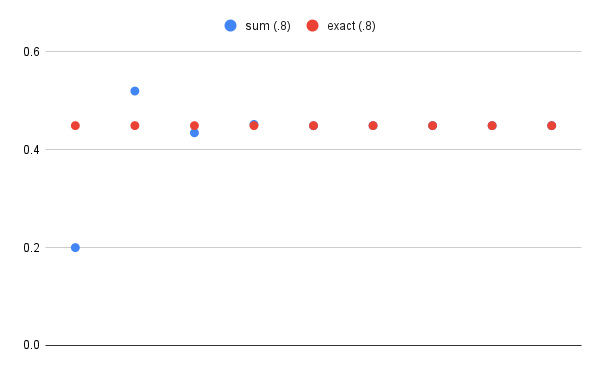
\includegraphics[scale=0.5]{img/chart.png}\]
\[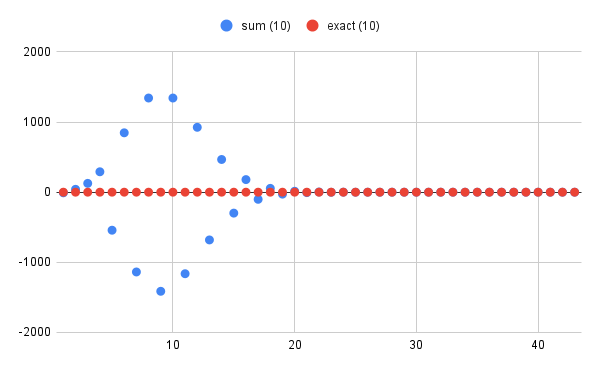
\includegraphics[scale=0.5]{img/chart1.png}\]
Clearly, there is a quick convergence towards the exact solution here, with nearly indistinguishable results at \(n=5\) in the first case and $n=20$ in the second.

For \(x=10\), part of the output of Program 1 appears below.

\begin{verbatim}

[dwilk14@tigers ~/Project2]$ ./dwilk14_proj2p1
Input a (floating point) number:
10
n: 1, element: -10, sum: -9, exact: 4.53999e-05
n: 2, element: 50, sum: 41, exact: 4.53999e-05
n: 3, element: -166.667, sum: -125.667, exact: 4.53999e-05
n: 4, element: 416.667, sum: 291, exact: 4.53999e-05
n: 5, element: -833.333, sum: -542.333, exact: 4.53999e-05
n: 6, element: 1388.89, sum: 846.555, exact: 4.53999e-05
n: 7, element: -1984.13, sum: -1137.57, exact: 4.53999e-05
n: 8, element: 2480.16, sum: 1342.59, exact: 4.53999e-05
n: 9, element: -2755.73, sum: -1413.14, exact: 4.53999e-05
n: 10, element: 2755.73, sum: 1342.59, exact: 4.53999e-05
n: 11, element: -2505.21, sum: -1162.62, exact: 4.53999e-05
n: 12, element: 2087.68, sum: 925.052, exact: 4.53999e-05

\end{verbatim}

Comparing \(n=9\) and \(n=10\), we can see that the corresponding terms are large and are almost exactly additive inverses of each other.

For small \(n\), the error is quite high. This is an approximation error, as the sum isn't given sufficient terms to converge very well.

\section{Program 2 Analysis}
\label{sec:orgf7f6b3d}

Below is a plot of the computed and exact solutions as a function of \(x\in[6, 10]\).
It is evident that the computed solution is excellent for the lower values $x$, but near $x=10$ the approximation becomes poor.
\[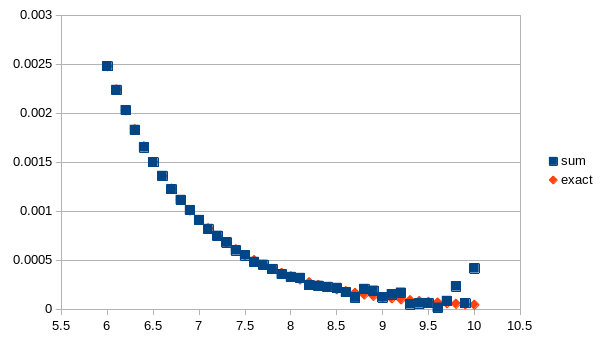
\includegraphics[scale=0.5]{img/chart3.png}\]

The absolute error as a function of \(N\) appears below.
\[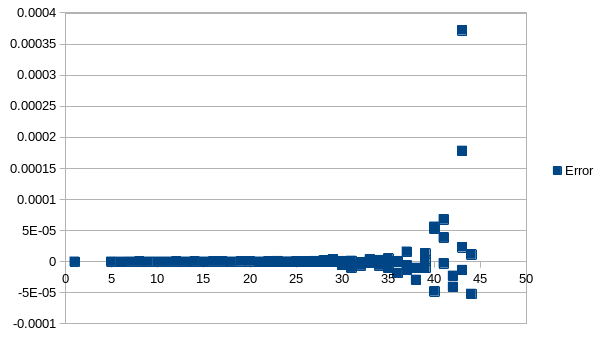
\includegraphics[scale=0.5]{img/chart4.png}\]
The error appears to increase with $N$, and this is due to the domination of the round-off error relative to the approximation error with the increased number of floating-point operations taking place.

\section*{Script Files}
\subsection{Program 1}
\begin{verbatim}
Script started on Tue 14 Sep 2021 06:46:23 PM CDT
tput: unknown terminal "st-256color"
tcsh: No entry for terminal type "st-256color"
tcsh: using dumb terminal settings.
[dwilk14@tigers ~/Project2]$ cat dwilk14_proj2p1.cpp
#include <iostream>
#include <fstream>
#include <cmath>

using namespace std;

int main() {
  float error, sum, element, exact, x;

  error = 1e-6;

  cout << "Input a (floating point) number: " << endl;
  cin >> x;

  sum = 1.;
  element = 1.;
  exact = exp(-x);

  int n = 0;
  do {
    ++n;
    element *= -x/n;
    sum += element;
    cout << "n: " << n << ", element: " << element << ", sum: " << sum << ", exact: " << exact << endl;
  } while (sum == 0 || fabs(element / sum) > error);


  return 0;

}
[dwilk14@tigers ~/Project2]$ g++ dwilk14_proj2p1.cpp -o dwilk14_proj2p1
[dwilk14@tigers ~/Project2]$ ./dwilk14_proj2p1
Input a (floating point) number:
10
n: 1, element: -10, sum: -9, exact: 4.53999e-05
n: 2, element: 50, sum: 41, exact: 4.53999e-05
n: 3, element: -166.667, sum: -125.667, exact: 4.53999e-05
n: 4, element: 416.667, sum: 291, exact: 4.53999e-05
n: 5, element: -833.333, sum: -542.333, exact: 4.53999e-05
n: 6, element: 1388.89, sum: 846.555, exact: 4.53999e-05
n: 7, element: -1984.13, sum: -1137.57, exact: 4.53999e-05
n: 8, element: 2480.16, sum: 1342.59, exact: 4.53999e-05
n: 9, element: -2755.73, sum: -1413.14, exact: 4.53999e-05
n: 10, element: 2755.73, sum: 1342.59, exact: 4.53999e-05
n: 11, element: -2505.21, sum: -1162.62, exact: 4.53999e-05
n: 12, element: 2087.68, sum: 925.052, exact: 4.53999e-05
n: 13, element: -1605.9, sum: -680.852, exact: 4.53999e-05
n: 14, element: 1147.07, sum: 466.222, exact: 4.53999e-05
n: 15, element: -764.716, sum: -298.494, exact: 4.53999e-05
n: 16, element: 477.948, sum: 179.454, exact: 4.53999e-05
n: 17, element: -281.146, sum: -101.692, exact: 4.53999e-05
n: 18, element: 156.192, sum: 54.5, exact: 4.53999e-05
n: 19, element: -82.2064, sum: -27.7064, exact: 4.53999e-05
n: 20, element: 41.1032, sum: 13.3968, exact: 4.53999e-05
n: 21, element: -19.5729, sum: -6.17617, exact: 4.53999e-05
n: 22, element: 8.89679, sum: 2.72062, exact: 4.53999e-05
n: 23, element: -3.86817, sum: -1.14755, exact: 4.53999e-05
n: 24, element: 1.61174, sum: 0.464186, exact: 4.53999e-05
n: 25, element: -0.644695, sum: -0.180509, exact: 4.53999e-05
n: 26, element: 0.24796, sum: 0.0674506, exact: 4.53999e-05
n: 27, element: -0.0918369, sum: -0.0243863, exact: 4.53999e-05
n: 28, element: 0.0327989, sum: 0.00841258, exact: 4.53999e-05
n: 29, element: -0.01131, sum: -0.00289739, exact: 4.53999e-05
n: 30, element: 0.00376999, sum: 0.0008726, exact: 4.53999e-05
n: 31, element: -0.00121613, sum: -0.000343526, exact: 4.53999e-05
n: 32, element: 0.000380039, sum: 3.65134e-05, exact: 4.53999e-05
n: 33, element: -0.000115163, sum: -7.865e-05, exact: 4.53999e-05
n: 34, element: 3.38716e-05, sum: -4.47784e-05, exact: 4.53999e-05
n: 35, element: -9.6776e-06, sum: -5.4456e-05, exact: 4.53999e-05
n: 36, element: 2.68822e-06, sum: -5.17678e-05, exact: 4.53999e-05
n: 37, element: -7.26546e-07, sum: -5.24943e-05, exact: 4.53999e-05
n: 38, element: 1.91196e-07, sum: -5.23031e-05, exact: 4.53999e-05
n: 39, element: -4.90247e-08, sum: -5.23521e-05, exact: 4.53999e-05
n: 40, element: 1.22562e-08, sum: -5.23399e-05, exact: 4.53999e-05
n: 41, element: -2.98931e-09, sum: -5.23429e-05, exact: 4.53999e-05
n: 42, element: 7.11741e-10, sum: -5.23421e-05, exact: 4.53999e-05
n: 43, element: -1.65521e-10, sum: -5.23423e-05, exact: 4.53999e-05
n: 44, element: 3.76185e-11, sum: -5.23423e-05, exact: 4.53999e-05
[dwilk14@tigers ~/Project2]$ cp dwilk14_proj2p1.txt /home3/kristina/phys2411/.
[dwilk14@tigers ~/Project2]$ exit
exit

Script done on Tue 14 Sep 2021 06:48:41 PM CDT

\end{verbatim}
\subsection{Program 2}
\begin{verbatim}
Script started on Tue 14 Sep 2021 06:51:35 PM CDT
tput: unknown terminal "st-256color"
tcsh: No entry for terminal type "st-256color"
tcsh: using dumb terminal settings.
[dwilk14@tigers ~/Project2]$ cat dwilk14_proj2p2.cpp
#include <cmath>
#include <iostream>
#include <fstream>

using namespace std;

int main() {
  float error, xmin, xmax, xstep, sum, element, exact, x;
  ofstream outfile("p2_out.txt");

  error = 1e-6;
  xmin = 0.; xmax = 10.0; xstep = 0.1;

  x = xmin;
  outfile << "n\tx\tsum\texact\tsum-exact" << endl;
  while (x < xmax + 0.5 * xstep) {
    sum = 1.;
    element = 1.;
    exact = exp(-x);

    int n = 0;
    do {
        ++n;
        element *= -x/n;
        sum += element;
    } while (sum == 0 || fabs(element / sum) > error);


    outfile << n << " " << x << " " << sum << " " << exact << " " << sum - exact << endl;

    x += xstep;
  }

  return 0;

}

[dwilk14@tigers ~/Project2]$ g++ dwilk14_proj2p2.cpp -o dwilk14_proj2p2
[dwilk14@tigers ~/Project2]$ ./dwilk14_proj2p2
[dwilk14@tigers ~/Project2]$ cp dwilk14_proj2p2.txt /home3/kristina/phys2411/.
[dwilk14@tigers ~/Project2]$ exit
exit

Script done on Tue 14 Sep 2021 06:54:09 PM CDT

\end{verbatim}
\end{document}
%%% Local Variables:
%%% mode: latex
%%% TeX-master: t
%%% End:

